As explained in Section~\ref{sec:intro} OpenMP 4.0 provides two environment variables OMP\_PROC\_BIND and OMP\_PLACES to help users define the thread placement for their shared memory OpenMP application which together we refer to as \textit{OpenMP Affinity}.%
%\begin{figure}[h!]
%  \centering
%  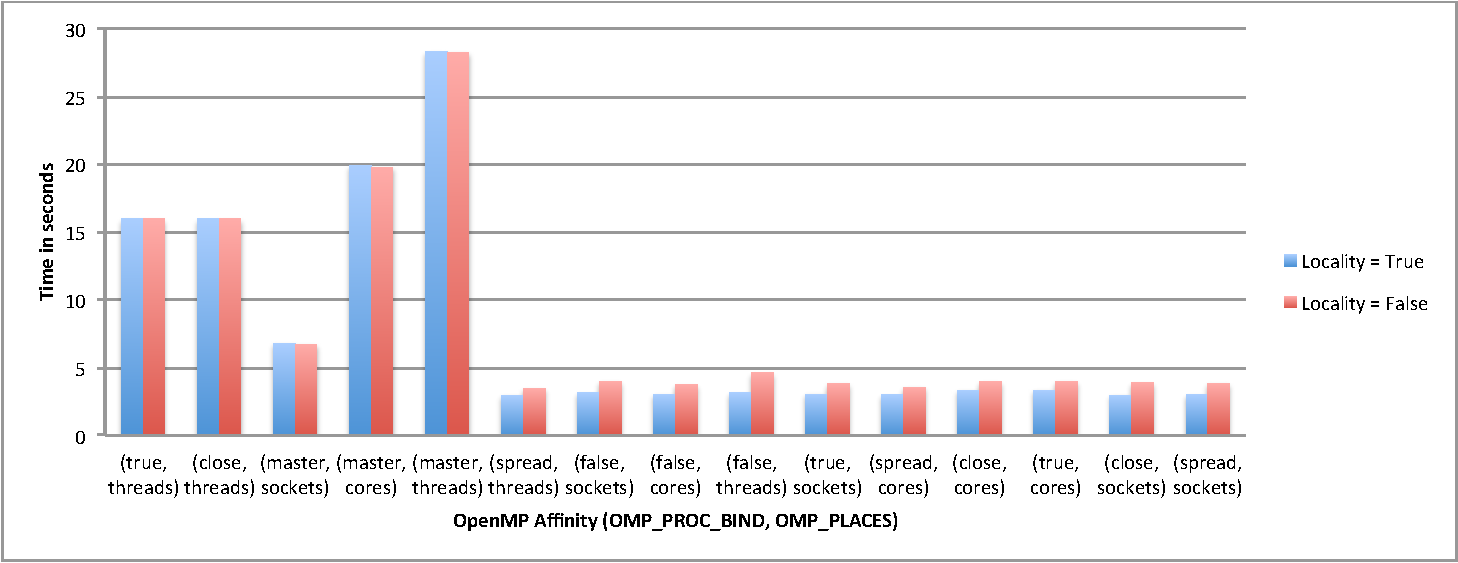
\includegraphics[height=0.4\textwidth, width=0.8\textwidth]{./Images/10Perf.pdf}
%       \caption{Performance with 10 OpenMP threads on \textit{Crest}}
%       \label{fig:10th}
%\end{figure}
%
 We experiment with the locality aware and locality unaware versions of the Jacobi program along with the default first-touch policy to observe the behavior over varying number of threads. 
 For each thread count we record the POWER8 hardware counters and the placement of the threads on the hardware. 
 Figure~\ref{fig:20th} shows the performance of 20 OpenMP threads with different OpenMP Affinity settings. We observed similar results for 10, 40, 80 and 160 OpenMP threads and hence do not show them here.
%
\begin{figure}[h!]
  \centering
  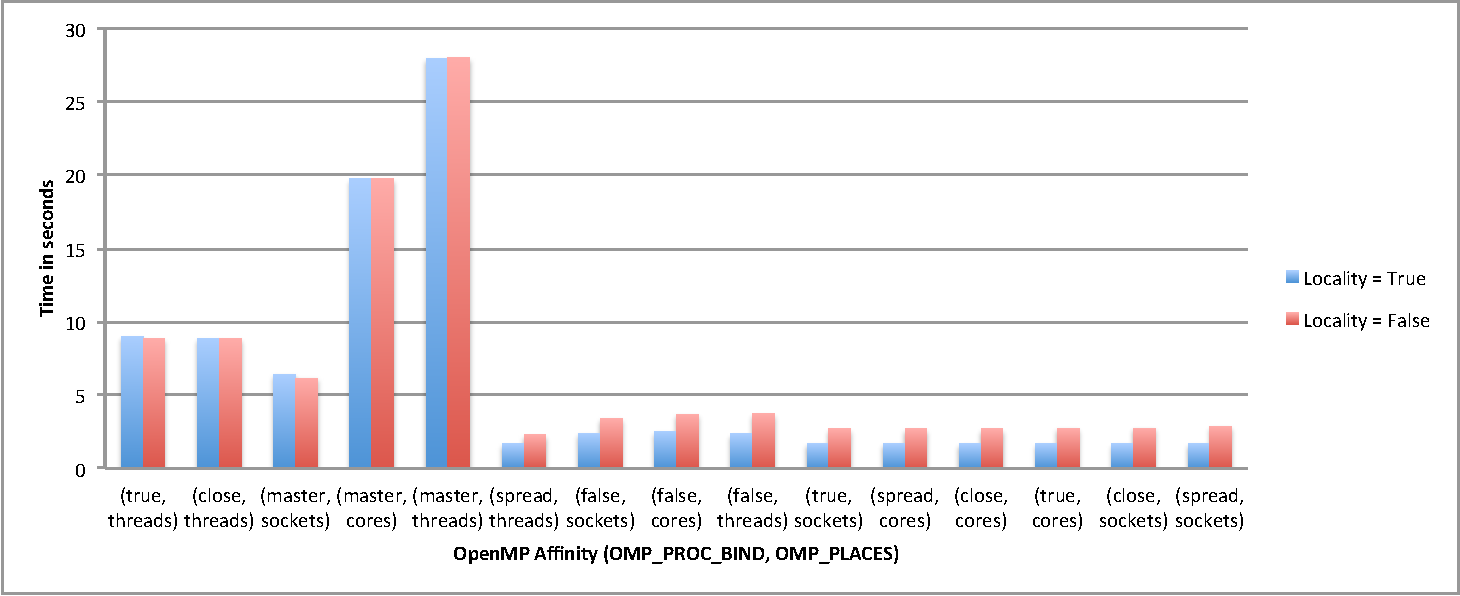
\includegraphics[height=0.4\textwidth, width=0.95\textwidth]{./Images/20Perf.pdf}
       \caption{Performance with 20 OpenMP threads on \textit{Crest}}
       \label{fig:20th}
\end{figure}
%
\begin{figure}[h!]
  \centering
  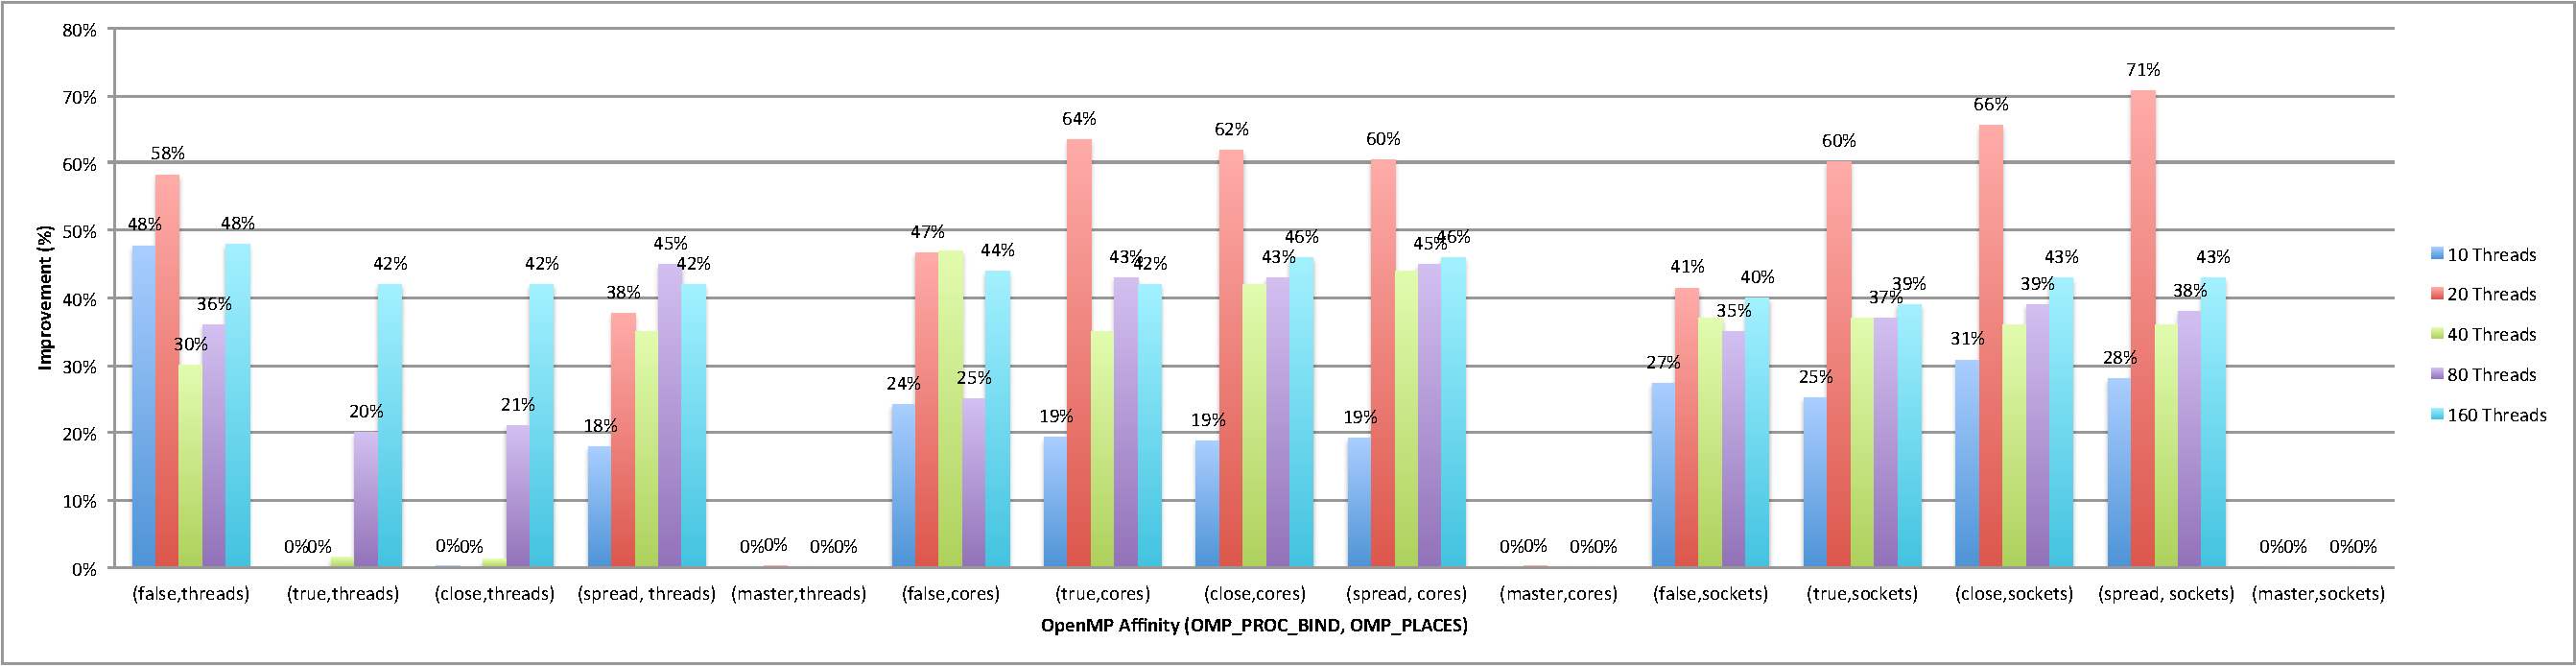
\includegraphics[height=0.4\textwidth, width=0.95\textwidth]{./Images/ImpAll.pdf}
       \caption{Comparing Performance Improvement between different number of OpenMP threads}
       \label{fig:imp}
\end{figure}
Figure~\ref{fig:imp} shows the improvement of the locality aware versions of the Jacobi program over the locality unaware version when using different OpenMP Affinity setting for different OpenMP thread counts. 
For the \textit{(master, threads)} configuration all threads execute on CPUID 0. 
All threads execute in the same core as the master when the configuration is set to \textit{(master, core)}, similarly for \textit{(master, socket)} all threads execute in the same socket. In this case all threads are executing on CPUs 0 through 79 which corresponds to a single NUMA domain. When OMP\_PROC\_BIND set to master we see in Figure ~ref{fig:Imp} that there is no improvement of locality aware algorithms over non-locality aware algorithms (both using the first-touch policy).
For \textit{(close, threads)}, we observe that all OpenMP threads execute on random CPUs between 0-19. All of these cases don't suffer from memory locality issues because they access memory local to the memory within the chip.
In the \textit{(spread, sockets)} and \textit{(close, sockets)} configuration threads are spread across sockets but may be mapped to the same core. We observed that the \textit{(true, threads)} configuration is equivalent to the \textit{(close,threads)} according to the thread mappings.
For all OpenMP affinity settings  with OMP\_PROC\_BIND set to false, threads can migrate and are not bound to a specific thread, core or socket. This migration makes it less impactful on the data placement, but suffers from degraded performance.
\begin{figure}[h!]
  \centering
  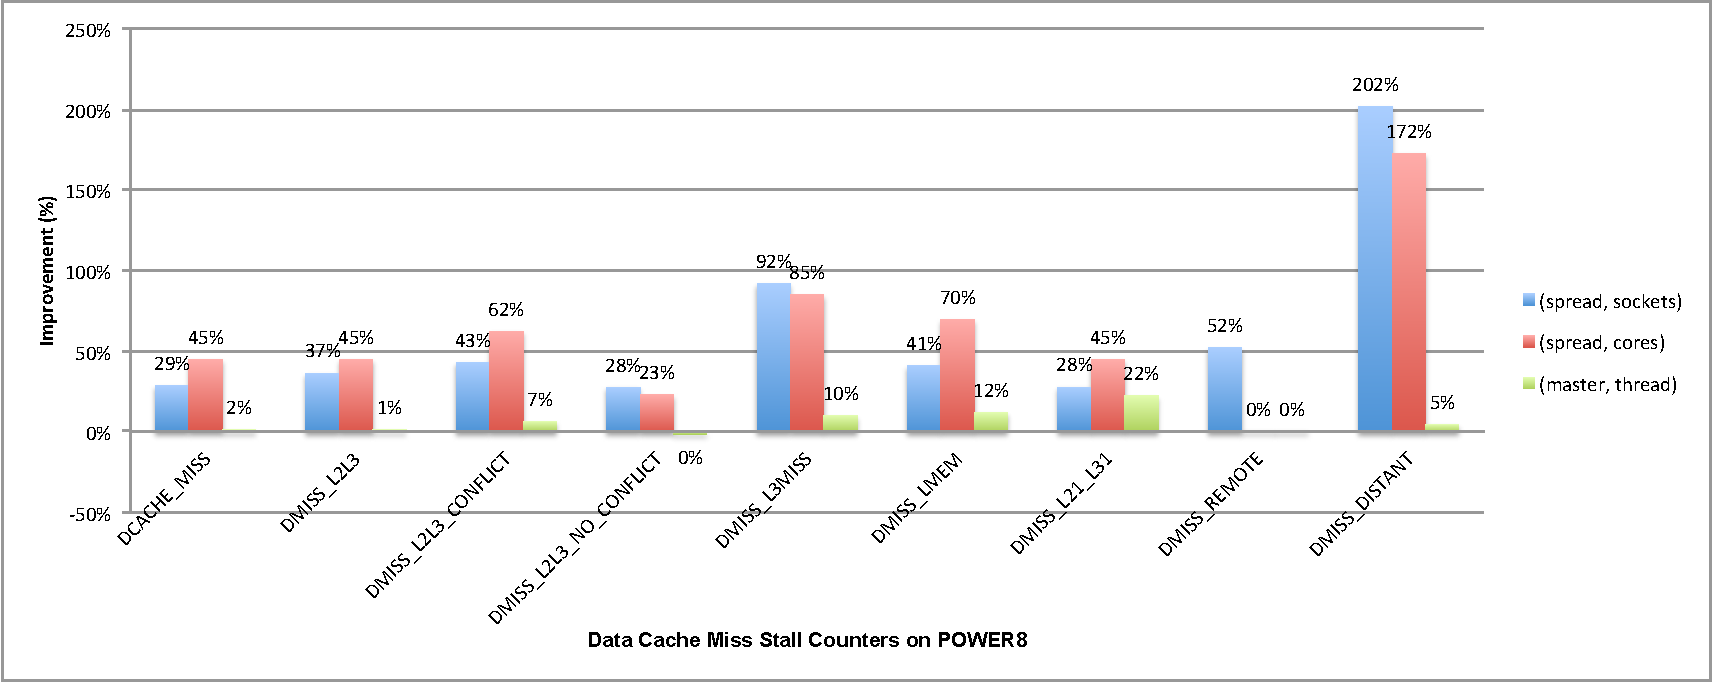
\includegraphics[height=0.4\textwidth, width=0.95\textwidth]{./Images/HW.pdf}
       \caption{Comparing Hardware Counter Change}
       \label{fig:HW}
\end{figure}
%
%Hardware Counter notes
Next we look at the hardware counters on the POWER8 system corresponding to the different configurations. 
We select the three cases of OpenMP Affinity tuple that represent the best, mid and worst improvement as seen in Figure~\ref{fig:imp}. 
%the cases where we see more improvement for data locality on a given affinity setting 
Selected cases are \textit{(spread, sockets)},  \textit{(spread, cores)}, and  \textit{(master, thread)}. For these cases we record the hardware counters for the locality aware and locality unaware versions and calculate the improvement as the value of their difference as a percentage of the value of the locality unaware hardware counter value. 
From Figure~\ref{fig:HW} we see that the two hardware counters that show the effects of data locality the most are DMISS\_DISTANT, DMISS\_L3MISS.
We would have expected to see more significant variation in the value of DMISS\_REMOTE, but we found that in some cases, these remote accesses can be cached.
For example, the case of \textit{(spread, sockets)} has better DMISS\_REMOTE improvement than  \textit{(spread, cores)}. 
In (spread, sockets) some threads (not all) are running on the same core sharing local cache lines for (L1, L2) and thus taking advantage of cache reuse for remote data access. 
This can also be seen by the significant improvement in DMISS\_DISTANT which quantifies the stalls by L1 reloads from distant interventions and memory. 
The improvements we see in  \textit{(spread, cores)} are more due to DMISS\_L21\_L31, which shows a better utilization of the L2/L3 cache as this hardware counter measures the stall cycles by Dcache miss which are resolved on chip. 
In the case of  \textit{(spread, cores)} we are effectively increasing the amount of 
L2 cache available to each OpenMP thread, as each thread has access to its own L2 cache on a given core. 
For the \textit{(master, thread)} case, there is very little improvement in the memory subsystem utilization as everything is running on the same thread and the most of the data is local to the socket. In this case the data-locality version does not make any difference. This is also true for the case  \textit{(close, threads)} where
 we don't see improvements on the data locality version since data is local to the threads.


